\documentclass{article}

\usepackage{array}
\usepackage{gensymb}
\usepackage{graphicx}
\usepackage{pgfplots}
\usepackage{siunitx}

\title{Determining the Effect of Ramp Incline on Acceleration}
\date{3 October 2014}
\author{Tarik Onalan}

\begin{filecontents}{data.dat}
    xVal   yVal     xDel  yDel
    0.6016 0.034414 0.075 0.003536
    1.249  0.1666   0.075 0.0019
    2.057  0.30314  0.075 0.00964
    2.981  0.4459   0.075 0.0048
    3.750  0.58386  0.075 0.00484
\end{filecontents}

\begin{document}
    \maketitle
    \section{Introduction}
    \section{Materials}
        \begin{enumerate}
            \item 1 Cart
            \item 1 Ramp
            \item 1 Ruler
            \item 1 Vernier Logger
            \item 1 Position Tracker
            \item 1 Computer
            \item 5 Books
        \end{enumerate}
    \section{Procedure}
        \begin{enumerate}
            \item Set up Vernier box with position logger
            \item Place one book on a flat surface
            \item Indicate a constant distance on the ramp
            \item Lay one end of the ramp on the book
            \item Place position logger on the elevated end of the ramp
            \item Place cart at beginning of indicated distance
            \item Let go of cart, track acceleration of cart
            \item Record average acceleration for the cart
            \item Repeat steps 2-7, iterating the book count (\(1\to5\))
        \end{enumerate}
    \section{Diagram}
        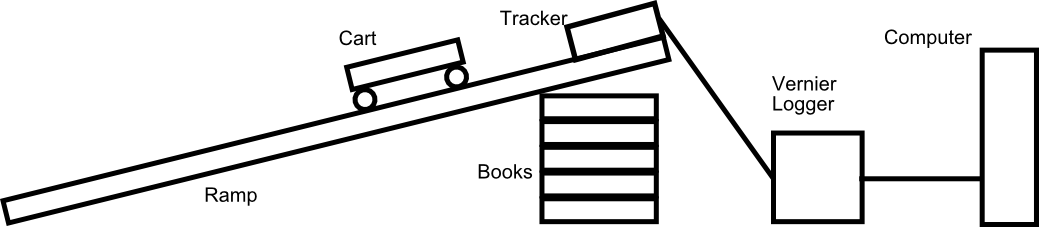
\includegraphics[width=\textwidth]{diagram}
    \section{Data}
        \noindent\resizebox{\textwidth}{!}{
            \Huge
            \begin{tabular}{|c|c||c|c|c|c|c|c|} \hline
                Height & Slope & Trial 1 & Trial 2 & Trial 3 & Trial 4 & Trial 5 & Average \\\hline
                \SI{1.5}{\cm} & \(0.6016\degree\) & \SI{0.03172}{\m\per\second\squared} & \SI{0.03257}{\m\per\second\squared} & \SI{0.03346}{\m\per\second\squared} & \SI{0.03795}{\m\per\second\squared} & \SI{0.03637}{\m\per\second\squared} & \SI{0.034414}{\m\per\second\squared} \\\hline
                \SI{3.1}{\cm} & \(1.249\degree\) & \SI{0.1659}{\m\per\second\squared} & \SI{0.1670}{\m\per\second\squared} & \SI{0.1683}{\m\per\second\squared} & \SI{0.1647}{\m\per\second\squared} & \SI{0.1671}{\m\per\second\squared} & \SI{0.1666}{\m\per\second\squared} \\\hline
                \SI{5.1}{\cm} & \(2.057\degree\) & \SI{0.3036}{\m\per\second\squared} & \SI{0.3099}{\m\per\second\squared} & \SI{0.3007}{\m\per\second\squared} & \SI{0.3080}{\m\per\second\squared} & \SI{0.2935}{\m\per\second\squared} & \SI{0.30314}{\m\per\second\squared} \\\hline
                \SI{7.4}{\cm} & \(2.981\degree\) & \SI{0.4492}{\m\per\second\squared} & \SI{0.4431}{\m\per\second\squared} & \SI{0.4485}{\m\per\second\squared} & \SI{0.4476}{\m\per\second\squared} & \SI{0.4411}{\m\per\second\squared} & \SI{0.4459}{\m\per\second\squared} \\\hline
                \SI{9.3}{\cm} & \(3.750\degree\) & \SI{0.5887}{\m\per\second\squared} & \SI{0.5813}{\m\per\second\squared} & \SI{0.5839}{\m\per\second\squared} & \SI{0.5808}{\m\per\second\squared} & \SI{0.5846}{\m\per\second\squared} & \SI{0.58386}{\m\per\second\squared} \\\hline\hline
                \multicolumn{8}{|c|}{Uncertainty}\\\hline
                \SI{0.05}{\cm} & \(0.075\degree\) & \SI{0.003536}{\m\per\second\squared} & \SI{0.0019}{\m\per\second\squared} & \SI{0.00964}{\m\per\second\squared} & \SI{0.0048}{\m\per\second\squared} & \SI{0.00484}{\m\per\second\squared} &\\\hline
            \end{tabular}
        }\\

        \begin{tabular}{|c|c|c|c|}
            \hline
            Start Point & End Point & Length of Track & Uncertainty \\\hline
            \SI{50}{\cm} & \SI{192.2}{\cm} & \SI{142.2}{\cm} & \SI{0.1}{\cm} \\
            \hline
        \end{tabular}

        \begin{tikzpicture}
            \begin{axis}[
                scale=1.75,
                title={Acceleration Relative to Ramp Incline},
                xlabel={Slope [\(\degree\)]},
                ylabel={Acceleration [\si{\m\per\second\squared}]},
                xmin=0.0, xmax=4.0,
                ymin=0.0, ymax=0.75,
                legend pos=north west,
                ymajorgrids=true,
                grid style=dashed
            ]
                \addplot[
                    color=blue,
                    mark=*,
                ] plot [
                    error bars/.cd,
                        x dir=both,
                        y dir=both,
                        x explicit,
                        y explicit
                ] table [
                    x=xVal,
                    y=yVal,
                    x error=xDel,
                    y error=yDel
                ]{data.dat};

                \addplot[
                    color=red,
                    domain=0:4,
                    mark=none
                ] {0.171249*x-0.0575874};

                \draw[
                    red,
                    thin
                ] (axis cs:0.5266,0.030878) rectangle (axis cs:0.6766,0.03795);

                \draw[
                    red,
                    thin
                ] (axis cs:1.174,0.1647) rectangle (axis cs:1.324,0.1685);

                \draw[
                    red,
                    thin
                ] (axis cs:1.982,0.2935) rectangle (axis cs:2.132,0.31278);

                \draw[
                    red,
                    thin
                ] (axis cs:2.906,0.4411) rectangle (axis cs:3.056,0.4507);

                \draw[
                    red,
                    thin
                ] (axis cs:3.675,0.57902) rectangle (axis cs:3.825,0.5887);

                \addlegendentry{Average}
                \addlegendentry{0.171249x-0.0575874}
            \end{axis}
        \end{tikzpicture}
\end{document}
